\documentclass[11pt,a4paper]{article}

\usepackage[T1]{fontenc}
\usepackage[utf8]{inputenc}
\usepackage{amsmath}
\usepackage{booktabs}
\usepackage{geometry}
\usepackage{graphicx}
\usepackage{hyperref}
\usepackage{siunitx}
\usepackage{xcolor}

\geometry{margin=25mm}
\graphicspath{{figures/chicane-1/}{figures/chicane-2/}}
\hypersetup{
  colorlinks=true,
  linkcolor=blue!55!black,
  urlcolor=blue!55!black,
  citecolor=blue!55!black
}
\sisetup{scientific-notation=true}

\title{OPAL to OPALX Chicane Regression Tests}
\author{OPALX development note}
\date{\today}

\begin{document}
\maketitle

\section{Purpose}

This note documents the consolidated chicane regression tests in
\texttt{sandbox/chicane}.  The directory contains two OPAL/OPALX pairs:
\begin{itemize}
  \item \texttt{chicane-1-opal.in} and \texttt{chicane-1-opalx.in}: a
        five-particle hard-edge probe used to check the longitudinal
        dispersion of a symmetric four-SBEND chicane.
  \item \texttt{chicane-2-opal.in} and \texttt{chicane-2-opalx.in}: a
        10000-particle manufactured-distribution comparison using the stat
        file quantities energy, energy spread, RMS beam sizes, RMS momenta,
        and RMS emittances.
\end{itemize}
The plotting script \texttt{plot\_chicane\_figures.py} reads the run outputs
from \texttt{runs/}, writes publication-quality figures to \texttt{figures/},
and writes numerical summaries to \texttt{summaries/}.  The \texttt{figures/}
directory is intentionally kept figure-only.

\section{Geometry}

Both tests use the same idealized C-shaped chicane:
\begin{align}
  L_b &= \SI{1.0}{m}, &
  \theta &= \SI{0.1}{rad}, &
  D &= \SI{1.5}{m}, &
  C &= \SI{2.0}{m}.
\end{align}
The four physical bend signs are
\[
  (+\theta,\,-\theta,\,-\theta,\,+\theta)
\]
when viewed as a positive horizontal survey excursion in \(+x\).
For an OPAL-compatible SBEND the input length is treated as the chord length,
therefore
\[
  \rho = \frac{L_b}{2\sin(\theta/2)}.
\]
The exit displacement of a positive survey bend is
\[
  \Delta x_b = \rho\left(1-\cos\theta\right), \qquad
  \Delta z_b = \rho\sin\theta .
\]
In an OPAL \texttt{ELEMEDGE} deck the number attached to a bend is the
longitudinal position of the bend entrance on the design orbit.  In an OPALX
explicit-pose deck, the coordinates \((X,Y,Z)\) attached to an analytic SBEND
are instead the position of the bend's local element frame.  For the SBENDs
used here that local frame is at the middle of the bend: it is reached by
following the design orbit through half of the bend angle from the entrance.
Thus the OPALX bend coordinates are not copied from the OPAL entrance
\texttt{ELEMEDGE}; they are the entrance point plus the half-bend survey
displacement.  For a positive survey bend this displacement is
\[
  \Delta x_{1/2} = \rho\left(1-\cos\frac{\theta}{2}\right), \qquad
  \Delta z_{1/2} = \rho\sin\frac{\theta}{2}.
\]
For the return bends the corresponding displacement, again written from the
bend entrance point to the OPALX bend frame, is
\[
  \Delta x_{r,1/2} = \rho\left(\cos\frac{\theta}{2}-\cos\theta\right), \qquad
  \Delta z_{r,1/2} = \rho\left(\sin\theta-\sin\frac{\theta}{2}\right).
\]
The outer drifts are tilted by \(\theta\), so their projected increments are
\[
  \Delta x_D = D\sin\theta, \qquad
  \Delta z_D = D\cos\theta .
\]

\section{Test 1: five-particle \(R_{56}\) probe}

The first test uses five particles with
\[
  \delta = \frac{p_z}{p_0} - 1
      \in \{-2, -1, 0, 1, 2\}\times 10^{-3},
  \qquad
  p_0 = 1957.950928190185 .
\]
The plotting script reads the final monitor H5 files and fits final local
\(z\) against the initial \(\delta\).  The transport coefficient is reported
as
\[
  R_{56} = -\frac{d z_{\mathrm{exit}}}{d\delta}.
\]
The small-angle hard-edge reference used for this chicane is
\[
  R_{56,\mathrm{ref}}
    \simeq
    -\theta^2\left(\frac{4L_b}{3}+2D\right)
    =
    -4.333333333333334\times 10^{-2}\,\mathrm{m}.
\]
The current generated summary gives
\[
  R_{56,\mathrm{OPALX}} = -4.334628766121465\times 10^{-2}\,\mathrm{m},
  \qquad
  R_{56,\mathrm{OPAL}} = -4.337546378253016\times 10^{-2}\,\mathrm{m}.
\]

\begin{figure}[htbp]
  \centering
  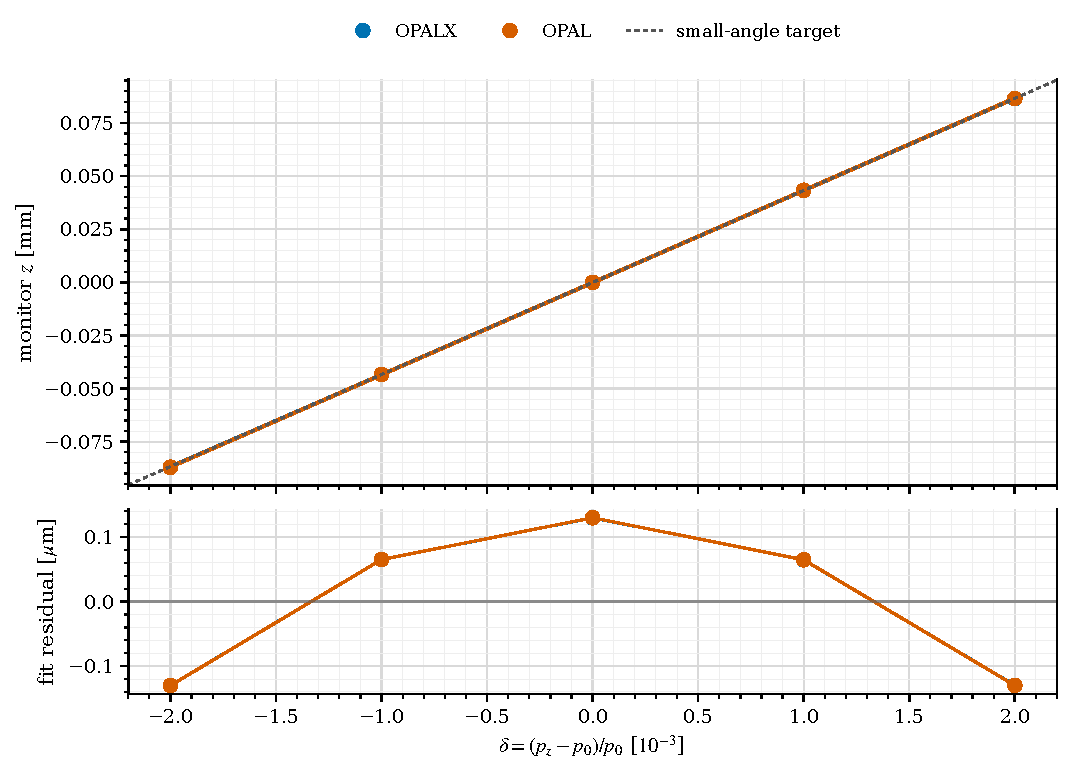
\includegraphics[width=0.92\linewidth]{chicane-1-r56.pdf}
  \caption{Five-particle \(R_{56}\) probe.  The top panel shows the fitted
  final monitor coordinate versus the input momentum offset.  The lower panel
  shows the fit residual.}
  \label{fig:r56}
\end{figure}

\section{Test 2: 10000-particle stat comparison}

The second test uses a deterministic manufactured distribution with
\(10^4\) particles, a \(\SI{5}{ps}\) time step, and a nonzero bunch charge.
The stat-file comparison deliberately ignores monitor files and compares only
quantities available in the OPAL and OPALX stat files.  OPAL samples are
interpolated onto the OPALX \(s\)-grid over the shared longitudinal interval.
For every quantity \(q\), the lower-panel relative difference is
\[
  |\Delta q|[\%]
     =
     100\,
     \frac{|q_{\mathrm{OPALX}}(s)-q_{\mathrm{OPAL}}(s)|}
          {|q_{\mathrm{OPAL}}(s)|}.
\]
Values with a denominator at numerical zero are masked.

\begin{figure}[htbp]
  \centering
  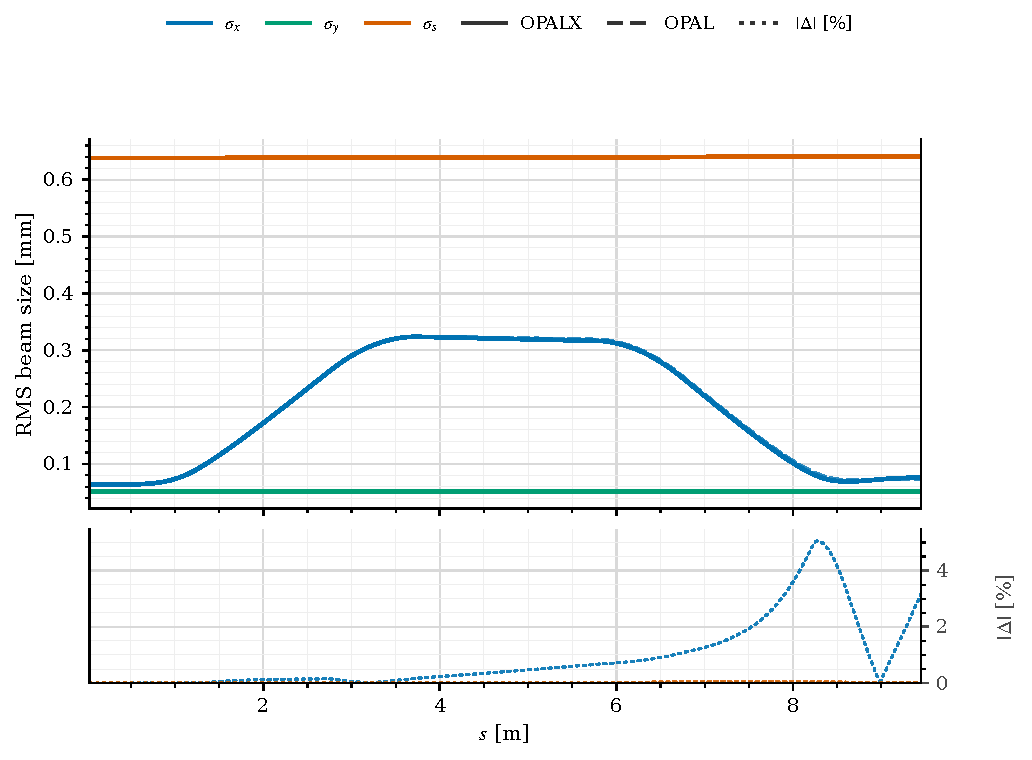
\includegraphics[width=0.92\linewidth]{stat_rms_relative_opalx_opal.pdf}
  \caption{RMS beam-size comparison from the stat files.}
  \label{fig:rms}
\end{figure}

\begin{figure}[htbp]
  \centering
  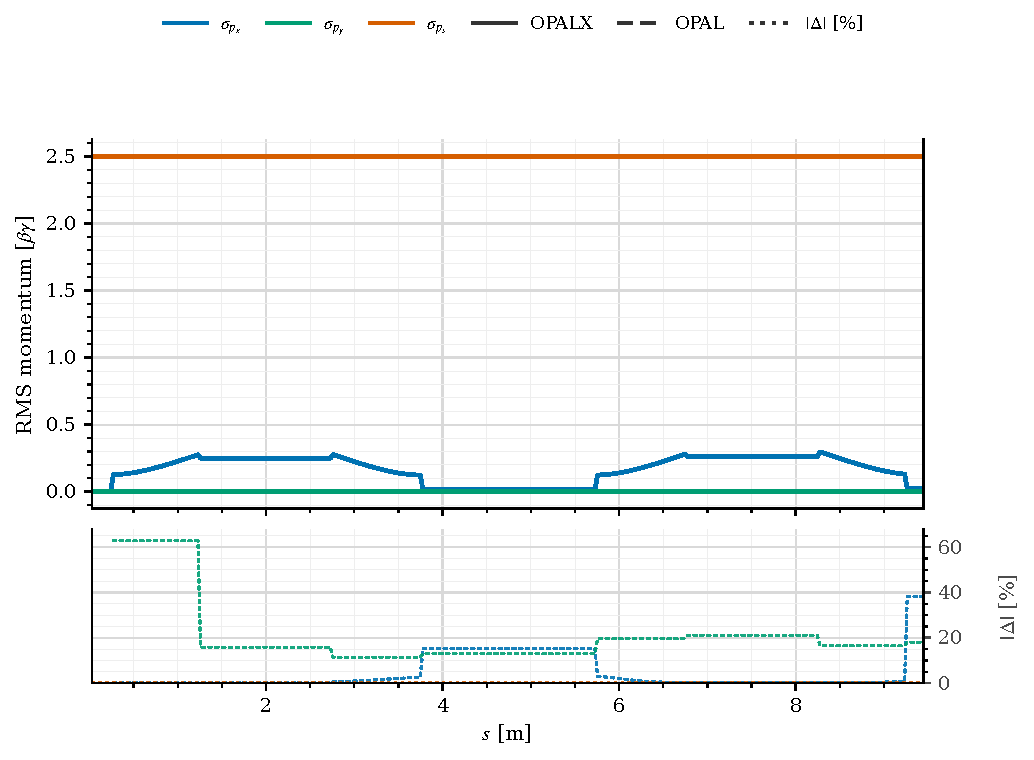
\includegraphics[width=0.92\linewidth]{stat_rms_momentum_relative_opalx_opal.pdf}
  \caption{RMS momentum comparison from the stat files.}
  \label{fig:momentum}
\end{figure}

\begin{figure}[htbp]
  \centering
  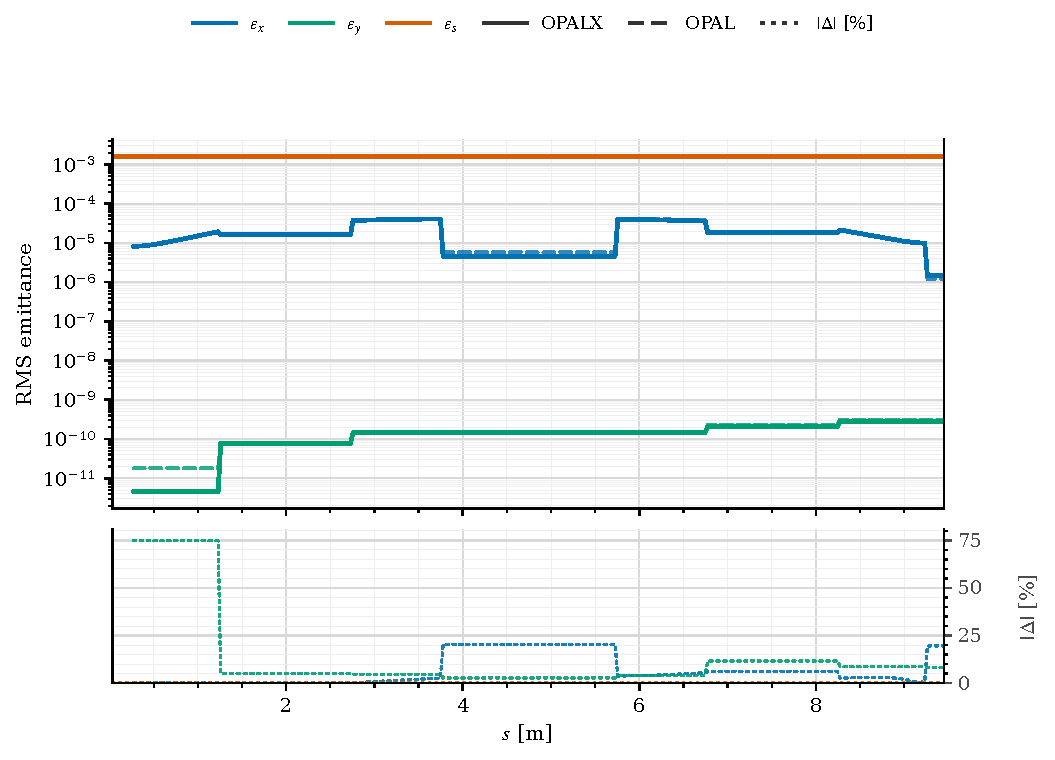
\includegraphics[width=0.92\linewidth]{stat_emittance_relative_opalx_opal.pdf}
  \caption{RMS emittance comparison from the stat files.  The emittance axis
  is logarithmic because the transverse and longitudinal emittances differ by
  many orders of magnitude.}
  \label{fig:emittance}
\end{figure}

\begin{figure}[htbp]
  \centering
  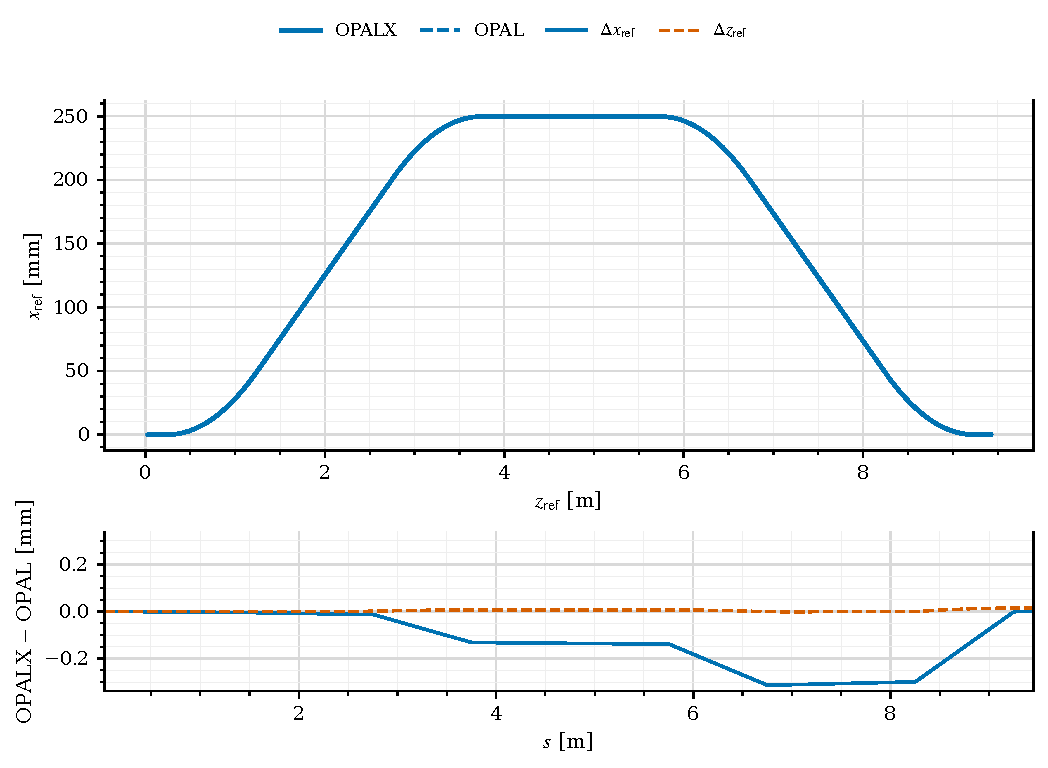
\includegraphics[width=0.92\linewidth]{stat_reference_xz_opalx_opal.pdf}
  \caption{Reference-orbit comparison and OPALX-minus-OPAL reference-orbit
  difference.}
  \label{fig:reference-orbit}
\end{figure}

\begin{figure}[htbp]
  \centering
  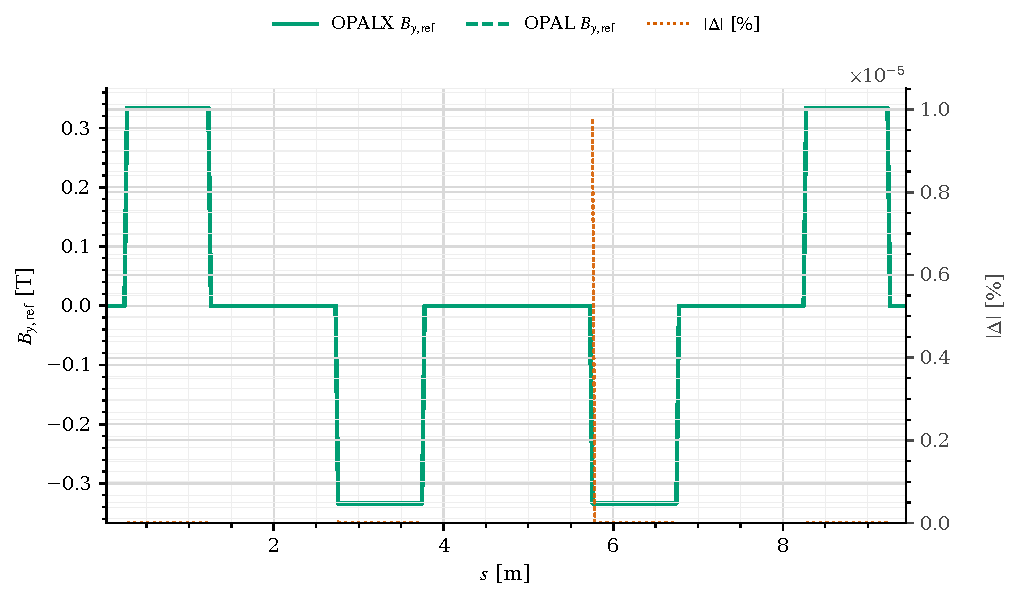
\includegraphics[width=0.92\linewidth]{stat_bfield_ref_opalx_opal.pdf}
  \caption{Reference-particle \(B_y\) comparison.  This plot is diagnostic:
  spikes at element interfaces are useful for checking placement and temporal
  crossing behavior, but the main beam comparison is based on stat-file RMS
  quantities.}
  \label{fig:by}
\end{figure}

\section{Moving an OPAL input deck to OPALX}

The chicane examples expose two different migration modes.  The first mode is
compatibility placement: keep the old OPAL reference-line \texttt{ELEMEDGE}
description and ask OPALX to interpret the deck as close as possible to OPAL.
The second mode is native OPALX placement: compute explicit element poses
\((X,Y,Z,\Theta,\Phi,\Psi)\) and place each element body in the global survey.

\subsection{Compatibility placement}

Use this mode when the goal is to reproduce an existing OPAL deck before
changing the lattice description.  The chicane-2 OPALX deck follows this
approach.
\begin{enumerate}
  \item Keep the OPAL element order and reference-line lengths.  For the
        chicane this is
        \[
          (\mathrm{DPRE}, B1, D12, B2, D23, B3, D34, B4, MEXIT).
        \]
  \item Keep \texttt{ELEMEDGE} values from OPAL:
        \[
        \begin{array}{ll}
          B1: & D_{\mathrm{pre}},\\
          B2: & D_{\mathrm{pre}} + L_b + D,\\
          B3: & D_{\mathrm{pre}} + 2L_b + D + C,\\
          B4: & D_{\mathrm{pre}} + 3L_b + 2D + C.
        \end{array}
        \]
  \item Keep OPAL bend model parameters that affect the old analytic field:
        \texttt{FMAPFN}, \texttt{DESIGNENERGY}, \texttt{FINT},
        \texttt{GAP}, and \texttt{HAPERT}.  In this hard-edge comparison
        \texttt{FINT=0} suppresses fringe focusing.
  \item Add \texttt{OPTION, IDEALIZED = TRUE;} when the purpose is an OPAL
        compatibility check.  This keeps the nominal design orbit on
        hard-edge reference-line lengths instead of applying
        profile-dependent path corrections during compatibility placement.
        The option is described in more detail below.
  \item Translate the OPAL fieldsolver names:
        \texttt{FSTYPE=NONE} becomes \texttt{TYPE=NONE};
        \texttt{MX,MY,MT} become \texttt{NX,NY,NZ};
        \texttt{PARFFTT} becomes \texttt{PARFFTZ}; and
        \texttt{BCFFTT} becomes \texttt{BCFFTZ}.
  \item Translate the distribution and beam setup.  OPAL uses
        \texttt{DISTRIBUTION} directly in \texttt{RUN}.  OPALX uses an
        \texttt{EMISSIONSOURCE}, an \texttt{EMISSIONSOURCELIST}, and a
        \texttt{BEAM} with \texttt{SOURCES}.  For a fixed from-file
        distribution, set \texttt{NPARTDIST} on the distribution and
        \texttt{NALLOC} on the beam.
  \item Translate the run method.  OPAL \texttt{METHOD="PARALLEL-T"} becomes
        OPALX \texttt{METHOD="PARALLEL"}.
\end{enumerate}

\subsection{Meaning of \texttt{IDEALIZED=TRUE}}

\texttt{IDEALIZED} is a global OPALX option used by the compatibility
placement compiler.  In the current code path it affects bends that do not
already have an explicit body pose.  That is, it acts on OPAL-style elements
placed by \texttt{ELEMEDGE}; it does not move elements whose placement is
already fixed by \((X,Y,Z,\Theta,\Phi,\Psi)\).

The compatibility-placement algorithm constructs a design orbit from the
OPAL-style sequence of \texttt{ELEMEDGE} anchors.  This is the same accelerator
language used in introductory beam-dynamics treatments: particle coordinates
are described in a local frame attached to the design orbit followed by the
design particle.  For an element whose OPAL-style entrance coordinate is
\[
  s_i = \texttt{ELEMEDGE}_i ,
\]
the straight drift from the previous element end to this entrance is taken as
\[
  \Delta s_i = s_i - s_{\mathrm{design,end},i-1}.
\]
After placing a bend, OPALX must choose the design-orbit path length used to
advance the reference-line end position to the next element.  Denote this
length by \(\ell_{\mathrm{place}}\).  The design-orbit update is
\[
  s_{\mathrm{design,end},i} = s_i + \ell_{\mathrm{place}} .
\]

With \texttt{IDEALIZED=TRUE}, OPALX uses the hard-edge design length for this
design-orbit advance:
\[
  \ell_{\mathrm{place}} = \ell_{\mathrm{hard}} .
\]
For an ideal sector bend this is the usual arc length
\[
  \ell_{\mathrm{hard}} = \rho |\theta|,
\]
while the body displacement used for the 3D placement is still the chord
geometry
\[
  \mathbf c
    =
    L_{\mathrm{chord}}\,
    R_{\mathrm{axis}}\!\left(\frac{\theta}{2}\right)\,\hat{\mathbf z}.
\]
For the chicane compatibility deck this means the next \texttt{ELEMEDGE}
anchor is interpreted exactly on the hard-edge OPAL reference line.  This is
the intended mode for reproducing an old OPAL input before introducing native
OPALX body poses.

With \texttt{IDEALIZED=FALSE}, OPALX replaces the hard-edge design-orbit
advance by a profile-dependent length derived from the bend design path.  In
the code this is
\[
  \ell_{\mathrm{place}}
    =
    \ell_{\mathrm{true}}
    - d_{\mathrm{entry}}
    - d_{\mathrm{exit}},
\]
where \(\ell_{\mathrm{true}}\) is the path length of the computed design path
over the field support, and
\[
  d_{\mathrm{entry}} = \|\mathbf r_{\mathrm{true}}(s_{\min})\|,
\]
\[
  d_{\mathrm{exit}}
    =
    \left\|
      R_z\,\mathbf r_{\mathrm{true}}(s_{\max})
      -
      \mathbf r_{\mathrm{exit,HE}}
    \right\|.
\]
Here \(\mathbf r_{\mathrm{true}}\) is the bend design path in the local bend
chart, \(R_z\) is the configured bend rotation about the global \(z\)-axis,
and \(\mathbf r_{\mathrm{exit,HE}}\) is the hard-edge exit point.  In the
implementation the hard-edge exit vector is constructed as
\[
  \mathbf r_{\mathrm{exit,HE}}
    =
    L_{\mathrm{chord}}\,
    R_{\mathrm{axis}}\!\left(\frac{\theta}{2}-E_1\right)\,
    \hat{\mathbf z},
\]
with bend angle \(\theta\), entrance edge angle \(E_1\), chord length
\(L_{\mathrm{chord}}\), and effective bend axis
\(\mathrm{axis}=R_z(0,-1,0)\).

The practical consequence is that \texttt{IDEALIZED=FALSE} can shift the
downstream design-orbit end position when a bend has finite fringe-field
support or another non-hard-edge design-path correction.  That is useful when
the OPALX lattice should follow the effective field-supported design path.  It
is not the right setting for a strict OPAL \texttt{ELEMEDGE} compatibility
test, because old OPAL decks normally place the next element by the hard-edge
reference length written in the input.

\subsection{Native OPALX body-pose placement}

Use native placement when the goal is to exploit OPALX's more general lattice
model or to make the survey explicit.  This is the mode used by
\texttt{chicane-1-opalx.in}.
\begin{enumerate}
  \item Choose the entrance survey origin.  In the chicane-1 deck the entrance
        is \((X_0,Y_0,Z_0)=(0,0,0)\) with tangent along \(+z\).
  \item Convert every old \texttt{ELEMEDGE} into a physical survey position.
        Drifts and monitors are placed at their entrance or plane position.
        For these analytic SBENDs, OPALX \texttt{X/Y/Z} denotes the bend's
        local element frame at the middle of the bend, not the entrance point.
        Therefore the half-bend survey displacement above must be added to
        the entrance point obtained from the OPAL \texttt{ELEMEDGE}.
  \item Set the bend orientation explicitly.  For the positive survey
        convention used here, B1 and B4 have body angles
        \(\Theta=\pm\theta/2\) and B2/B3 are oriented to close the chicane
        according to the local tangent.  The monitor planes use the tangent
        angle at their location.
  \item Check the OPALX SBEND sign convention.  In the native body-pose
        chicane, the OPALX \texttt{ANGLE} sign is opposite to the positive-X
        survey convention: B1 and B4 use \texttt{ANGLE=-TH}; B2 and B3 use
        \texttt{ANGLE=TH}.
  \item Replace OPAL aperture/fringe fields with OPALX-native hard-edge
        settings when appropriate.  For this hard-edge regression,
        \texttt{HGAP=0} and \texttt{FINT=0} are used in the native OPALX
        deck.
  \item Place diagnostic monitors explicitly using \texttt{X/Y/Z} and
        \texttt{THETA/PHI/PSI}.  For the \(R_{56}\) test this is essential,
        because the final local monitor coordinate is fitted against the
        input momentum offset.
\end{enumerate}

\subsection{Quantities that need special attention}

\begin{itemize}
  \item \textbf{Longitudinal coordinate:} OPAL and OPALX do not necessarily
        write monitor crossings with identical temporal sampling.  For the
        10000-particle comparison the robust quantity is therefore the stat
        file sampled on the shared \(s\)-range.
  \item \textbf{Bend placement:} if OPAL and OPALX disagree at bend
        interfaces, inspect the reference-particle field plot and the
        reference-orbit difference before changing physics parameters.
  \item \textbf{Sampling:} \texttt{STATDUMPFREQ} controls the density of the
        stat comparison.  Values of 10 or 20 are useful for chicane-2; denser
        output is usually only needed for debugging.
  \item \textbf{Relative differences:} use the same denominator everywhere:
        OPAL interpolated onto the OPALX \(s\)-grid.  This avoids mixing
        sampling artifacts with physics differences.
\end{itemize}

\section{Reproducing the figures}

From the repository root, regenerate all figures and summaries with
\begin{verbatim}
PYTHONPYCACHEPREFIX=/private/tmp/opalx-pycache \
MPLCONFIGDIR=/private/tmp/opalx-matplotlib \
/Users/adelmann/.venv-h6/bin/python sandbox/chicane/plot_chicane_figures.py
\end{verbatim}
The script expects the run outputs to already exist under
\texttt{sandbox/chicane/runs}.  It does not rerun OPAL or OPALX.

\end{document}
